% for details https://github.com/alwynmathew/phd-thesis-cseiitp

%% PLEASE READ THE COMMENTS BEFORE DOING ANYTHING 
\documentclass[12pt, a4paper]{book} % Font size=12, a4 paper, both-side printing, and in a book format
\usepackage[intlimits]{amsmath}%
\usepackage{amsthm}
\usepackage{caption3}
\usepackage{graphicx}
\usepackage{latexsym}
\usepackage{thesis}
\usepackage{rotating}
\usepackage{wrapfig}  % for biography photo
% \usepackage{pstricks} % for table shading https://tex.stackexchange.com/a/68871/136315
\usepackage{colortab} % for table shading
%\usepackage[algoruled, algochapter, linesnumbered]{algorithm2e} % for algorithm writing
%\usepackage{indentfirst}  % for indent the first paragraph of any chapter
%\usepackage{makeidx}      % for making index at last in the thesis
%\makeindex                % for making index at last in the thesis
\allowdisplaybreaks[1]
\usepackage{gensymb}
\usepackage{amssymb}

\usepackage{tabularx}
\usepackage{blindtext}
\usepackage{amstext}
\usepackage{epstopdf}
\usepackage{dcolumn}
\usepackage{array,multirow}
\usepackage{tikz}
\usepackage{titlesec}
\titlespacing*{\subsection}
{0pt}{0.6\baselineskip}{0.6\baselineskip}
\titlespacing*{\section}
{0pt}{0.75\baselineskip}{0.75\baselineskip}
\titlespacing*{\subsubsection}
{0pt}{0.5\baselineskip}{0.5\baselineskip}

%\newtheorem{theorem}{Theorem}
%\newtheorem{condition}{Condition}
%\usepackage{sectsty}
%\chapterfont{\centering}
%\chaptertitlefont{\centering}
%\usepackage{titlesec}
%\titleformat{\chapter}[display]
%  {\normalfont\bfseries\LARGE}
%  {\chaptertitlename~\thechapter}{1pc}
%  {{\color{brown}\titlerule[2pt]}\vspace{1pc}\MakeUppercase}
%\titleformat{name=\chapter,numberless}[display]
%  {\normalfont\bfseries\LARGE}{}{1pc}
%  {\MakeUppercase}
% \usepackage{caption}
% \usepackage{subcaption}
  
% Uncomment the following block and comment the next block (both starting with '\usepackage[dvips...') when you need for final printout. However to submit the softcopy of the thesis comment the first block and uncomment the next block.

%%-------------------- 1st Block ----------------------------
\usepackage[dvips,
                bookmarks,
                bookmarksopen=true,
                bookmarksnumbered=true,
                breaklinks=true,
                linktocpage,
                backref,
                colorlinks=true,
                linkcolor=black,
                urlcolor=black,
                citecolor=black,
                anchorcolor=black,
                hyperindex=true,
                hyperfigures
                ]{hyperref} % added by Sandipan

\usepackage{backrefx}% added by Sandipan
%-------------------- 1st Block Ends-------------------------

%-------------------- 2nd Block -----------------------------
%\usepackage[dvips]{hyperref} % for link boxes
%\usepackage[dvipdfmx]{hyperref} % for dvi to pdf conversion
%\usepackage[driverfallback=dvipdfm]{hyperref}
% \usepackage[pdftex]{hyperref}
% \hypersetup{
%              bookmarks,
%              bookmarksopen=true,
%              bookmarksnumbered=true,
%              breaklinks=true,
%              linktocpage,
%              backref,
%              colorlinks=false, % false: boxed links; true: colored links
%              linkcolor=red,    % color of internal links
%              citecolor=green,  % color of links to bibliography
%              urlcolor=cyan,    % color of external links
%              hyperindex=true,
%              anchorcolor=blue,
%              hyperfigures
% }


%\usepackage{backrefx} % for citing the section/page_no of each reference in Bibliography
%\usepackage[all]{hypcap} % for showing the figure as well as its caption.

%%--------------------2nd Block Ends--------------------------

\setcaptionwidth{0.9\textwidth} % For caption width 'Caution: Don't Change otherwise you'll be in trouble to control the figure/Table captions.
%\usepackage[linewidth=1pt]{mdframed}
\usepackage{minibox}
%\usepackage{algorithm}
\usepackage{algpseudocode}
\usepackage{enumitem}

\usepackage{arydshln}
\usepackage{multirow}
\usepackage{calc}
\usepackage{verbatim}
\usepackage{bbding}
\usepackage{bbm}
\usepackage{soul}
\usepackage{dsfont}
\usepackage{mathrsfs}
\usepackage{mathtools}
\usepackage{xcolor}
\usepackage{fancyhdr,graphicx}

\usepackage[caption=false]{subfig}
%\usepackage[ruled]{algorithm2e}
\usepackage{algorithm} 
%\usepackage{algorithmic}  
%\usepackage[algo2e]{algorithm2e}
%\usepackage[latin1]{inputenc}
%\newtheorem{theorem}{Theorem}
\newcommand{\cmt}[1]{ }
\usepackage{lipsum}

\newcommand{\thesistitle}{Thesis Title}
\newcommand{\authorname}{My Name}
\newcommand{\authorrollno}{XX21CSXX}
\newcommand{\supervisorname}{Dr. X}
\linespread{1.5}
\usepackage[top=1.25in, bottom=1.25in, left=1in, right=1in]{geometry}

\begin{document}
% ------------ Starting of Preamble Pages---------------------
\pagenumbering{none}
\include{HeadTail/coverpage}
\cleardoublepage

\setcounter{page}{1}
\pagenumbering{roman}
	
\begin{titlepage}
    \centering
    % College Logo
 %   \includegraphics[width=0.5\textwidth]{path_to_svkm_logo} \\[1.5cm]
    
    {\large Shri Vile Parle Kelavani Mandal's \\[0.2cm]
    \textbf{DWARKADAS J. SANGHVI COLLEGE OF ENGINEERING} \\[0.2cm]
    (Autonomous College Affiliated to the University of Mumbai)} \\[0.5cm]
    
    \textbf{\Huge 
    TrustChain: Decentralized Identity Verification for Secure Access } \\[1cm]
    
    \onehalfspacing
    \textit{Submitted in partial fulfillment of the requirement \\ of the degree of}\\[0.5cm]
    
    \textbf{\Large Bachelor of Technology in \\ Computer Science and Engineering \\ (IoT and Cyber Security with BlockChain Technology)} \\[0.5cm]
    
    \textbf{\Large By} \\[0.5cm]
    \textbf{Hiren Darji  \hspace{1cm} 60019230114} \\[0.2cm]
    \textbf{Devarsh Chandiwade \hspace{1cm} 60019230112} \\[0.2cm]
    \textbf{Tushar Panchal \hspace{1cm} 60019230116} \\[0.2cm]
    \textbf{Meenakshi Chandra \hspace{1cm} 60019220126} \\[.2cm]
    \textbf{ \hspace{1cm} } \\[.2cm]

    \textit{\Large Under the guidance of} \\[0.2cm]
    \textbf{Prof. Swapnil Gharat  } %\\[.5cm]
    
    % University Logo
    
\includegraphics[width=0.2\textwidth]{Mulogo.jpeg} 
    
    \textbf{\Large University of Mumbai} 
    
    \textbf{A.Y. 2025 -- 2026}
    
\end{titlepage}
%\clearpage

\include{HeadTail/dedication}
%\clearpage

%\addcontentsline{toc}{chapter}{Certificate of Approval} 
%\include{HeadTail/Certificate_of_approval_DC} 
% After the viva-voce, change the file name to 'Certificate_of_approval.tex'


\addcontentsline{toc}{chapter}{Declaration}

\begin{titlepage}
   % \centering
    \vspace*{1cm}
    
    {\Large \begin{center}
        \textbf{DECLARATION}
    \end{center}}  \\
    


\vspace{1cm}

\onehalfspacing  % Set line spacing to 1.5

We declare that this written submission represents our ideas in our own words and where others’ ideas or words have been included, we have adequately cited and referenced the original sources. We also declare that we have adhered to all the principles of academic honesty and integrity and have not misrepresented or fabricated or falsified any idea/data/fact/source in our submission. We understand that any violation of the above will be a cause for disciplinary action by the institute and can also evoke penal action from the sources which have thus not been properly cited or from whom proper permission has not been taken, when needed.

\vspace{1cm}

\noindent
\textbf{Hiren Darji   (60019230114)} %\hfill \textbf{(Sign against the name)} 
\\[0.5cm]
\textbf{Devarsh Chandiwade (60019230112)} %\hfill \textbf{(Sign against the name)} 
\\[0.5cm]
\textbf{Tushar Panchal (60019230116)} %\hfill \textbf{(Sign against the name)} 
\\[0.5cm]
\textbf{Meenakshi Chandra (60019220126)} %\hfill \textbf{(Sign against the name)} 
\\[0.5cm]


\noindent
\textbf{Place: } DJSCE \\ \hfill \textbf{Date:}



\addcontentsline{toc}{chapter}{Certificate}
\thispagestyle{empty} 
\begin{minipage}{.1\linewidth}
\hspace*{-.8cm}
\includegraphics[height=2.5cm,width=2.5cm]{djlogo2.png}
\end{minipage}
\hspace{.2cm}
\begin{minipage}{.9\linewidth}
%\begin{flushleft}
{\large
{SVKM's Dwarkadas J. Sanghvi College of Engineering\\}
\Large{Department of Computer Science and Engineering \\ (IoT and Cyber Security with Block Chain Technology)\\}}


%\end{flushleft}
\end{minipage}

\vspace{1.0in}

\centerline{\Large{\bf Certificate}}
\vspace{1cm}
%\fontsize{14pt}{16.8pt}
%\begin{large}
\noindent
This is to certify that the project entitled “TrustChain: Decentralized Identity Verification for Secure Access” is a genuine work of “Hiren Darji”
(60019230114), “Devarsh Chandiwade” (60019230112), “Tushar Panchal” (60019230116) and  “Meenakshi Chandra” (60019220126)  submitted in the partial fulfillment of the requirement for the award
of the Bachelor of Technology in Computer Science and Engineering (IoT and Cyber Security with Block Chain Technology).
\vspace{1in}

\noindent
\makebox[\textwidth][c]{%
  \parbox{0.45\textwidth}{%
    \centering
    \textbf{Prof. Swapnil Gharat}\\
    Project Guide
  }%
}
\vspace{1in}

\noindent
\begin{minipage}[t]{0.48\textwidth}
\centering
\textbf{Dr. Narendra Shekokar}\\
Vice Principal\\
and Head of the Department
\end{minipage}
\hfill
\begin{minipage}[t]{0.48\textwidth}
\centering
\textbf{Dr. Hari Vasudevan}\\
Principal
\end{minipage}



\vspace{1in}
\noindent
%\hspace{3.1in}{Department of Information Technology}\\
Place: DJSCE \\
\noindent Date : 

\addcontentsline{toc}{chapter}{Approval Sheet}
\begin{titlepage}
    \vspace*{1cm}

    \begin{center}
        {\Large \textbf{APPROVAL SHEET}}
    \end{center}

    \vspace{1cm}

    \begin{center}
    \setstretch{1.5}
    Project entitled, \textit{\textbf{“TrustChain: Decentralized Identity Verification for Secure Access”}}, submitted by \textbf{“Hiren Darji” (60019230114), “Devarsh Chandiwade” (60019230112), “Tushar Panchal” (60019230116)} and \textbf{“Meenakshi Chandra” (60019220126)} is approved for the award of the Bachelor of Technology in Computer Science and Engineering (Internet of Things and Cyber Security with Blockchain Technology).
    \end{center}

    \vspace{2cm}

    \noindent
    \begin{minipage}[t]{0.45\textwidth}
        \centering
        \textbf{Internal Examiner} \\
        Name and Signature
    \end{minipage}
    \hfill
    \begin{minipage}[t]{0.45\textwidth}
        \centering
        \textbf{External Examiner} \\
        Name and Signature
    \end{minipage}

    \vspace{2.5cm}

    \noindent
    \begin{minipage}[t]{0.45\textwidth}
        \centering
        \textbf{Prof. Swapnil Gharat} \\
        Project Guide
    \end{minipage}
    \hfill
    \begin{minipage}[t]{0.45\textwidth}
        \centering
        \textbf{Dr. Narendra Shekokar} \\
        Head of the Department
    \end{minipage}

    \vspace{2.5cm}

    \begin{center}
        \textbf{Dr. Hari Vasudevan} \\
        Principal
    \end{center}

    \vspace{1cm}

    \noindent
    \textbf{Place:} DJSCE \hspace{3cm} \\
    \textbf{Date:} \hspace{3cm} 

\end{titlepage}


\addcontentsline{toc}{chapter}{Acknowledgement}


\begin{titlepage}
   % \centering
    \vspace*{1cm}
    
    {\Large \begin{center}
        \textbf{Acknowledgement}
    \end{center}} } \\[1.5cm]

% We are sincerely thankful to Dwarkadas J Sanghvi College of Engineering for providing
% us with the opportunity to conduct research on the project titled "Medchain"
% We express our gratitude and deepest appreciation to our mentor, Prof. Dipali Bhole, who has assisted us in conducting the research for this project and guided us through each stage.
We take this opportunity to express our deep sense of gratitude to our project guide Prof. Swapnil Gharat for his continuous guidance and encouragement throughout the duration of our project work. It is because of his experience and wonderful knowledge we were able to fulfil the requirement for the completion of this project within the stipulated time. We would also like to thank Dr. Narendra Shekokar, Vice Principal and Head of the Department Computer Science and Engineering (IoT and Cyber Security with Block Chain Technology) for his encouragement, whole-hearted cooperation and support.

We would also like to thank our Principal, Dr. Hari Vasudevan and the management of D.J. Sanghavi College of Engineering, Vile Parle (W), Mumbai for providing us with all the facilities and a work-friendly environment. We acknowledge by thanking the assistance provided by departmental staff, library, lab assistant lab attendants.
% We have learned extensively about different deep learning architectures, including DNNs, RNNs, and transformers, and their applications in cryptanalysis. This project has 
% deepened our understanding of both cryptographic vulnerabilities and the potential of 
% deep learning in identifying these weaknesses. We hope that this paper provides valuable 
% insights into the intersection of cryptanalysis and deep learning, contributing to the 
% ongoing discourse in cybersecurity. I would also like to thank all the project members.

\vspace{1cm}

\noindent
\textbf{Hiren Darji (60019230114)} \\
\textbf{Devarsh Chandiwade (60019230112)} \\
\textbf{Tushar Panchal  (60019230116)} \\
\textbf{Meenakshi Chandra (60019220126)} \\



%%%%%%%%%%%%%%% LIST OF ABBREVIATIONS %%%%%%%%%%%%%%%%%%
	% \addcontentsline{toc}{chapter}{List of Abbreviations}
	% \markboth{List of Abbreviations}{List of Abbreviations}
	% % Give Abbreviations alphabetically
\chapter*{Abbreviations}\label{LstAbb} 

\begin{flushleft}
\begin{longtable}{lp{11cm}}
	
DID & Decentralized Identity \\
IPFS & InterPlanetary File System\\
ZKP & Zero-Knowledge Proof\\
DI & Decentralized Identity \\
RBAC & Role Based Access Control \\
UI & User Interface \\
UX & User Experience\\
SSI & Self Sovereign Identity\\
PoA & Proof of Authority\\
API & Application Programming Interface\\
NFT & Non-Fungible Token\\
JWT & JSON Web Token\\
KYC & Know Your Customer\\
PII & Personally Identifiable Information\\
AES & Advanced Encryption Standard\\
RSA & Rivest Shamir Adleman (Asymmetric Encryption Algorithm)\\
MFA & Multi-Factor Authentication\\
OTP & One-Time Password\\
DB & Database\\
DID Auth & Decentralized Identity Authentication\\
ISCC & International Symposium on Computers and Communications\\

\end{longtable}
\end{flushleft}

	% \clearpage{\pagestyle{empty}\cleardoublepage}

%%%%%%%%%%%%%%%%% LIST OF SYMBOLS %%%%%%%%%%%%%%%%%%%%%
 %   \addcontentsline{toc}{chapter}{List of Symbols}
	% \markboth{List of Symbols}{List of Symbols}
	% % % Greek Symbols are to be given first followed by other symbols alphabatically
% \chapter*{List of Notations and Operations}\label{LstSym}

% \begin{flushleft}
% \begin{longtable}{lp{12cm}}
	
% $X$ & Unknown 1\\
% $\mathcal{K}_0$ & Unknown 2\\
% $\epsilon$ & Permittivity of air \\

% \end{longtable}
% \end{flushleft}


	% \clearpage{\pagestyle{empty}\cleardoublepage}

%%%%%%%%%%%%%%%%%%%%%%%%%%%%%%%%%%%%%%%%%

\addcontentsline{toc}{chapter}{Abstract}
\chapter*{Abstract}
\sloppy

\vspace{1cm}
\par Government Identity documents have become groundwork for citizen verification, financial inclusion and public service. However unauthorized disclosure, fraudulent access and frequent misuse of individual's personal information expose gaps in routine verification and wrongful disbursement of welfare benefits which asks the immediate need for a more secure privacy holding approach. Existing infrastructure like DigiLocker takes care of the secure transmission but a factor of privacy exposure is still compromised. The proposed model introduces TrustChain based on blockchain framework for decentralized identify verification and secure access. The inducement shifts focus from submission of identity information to authentication by the means of DID (Decentralized Identifiers) ensuring that some personal information will be hidden to the document requestor. By integrating self sovereign identity principles, distributed storage and cryptographic operations the model enables users to authenticate without revealing personal parameters minimizing the risks of identity compromise. Pilot findings are particular not to mention that identity exposure is mitigated by such a representation and offers scalability towards integration into the current infrastructures such as Aadhaar connected services and Digital locker. A safe identity space where individuals retain ownership to personal information as organizations and governments achieve acceptable validation. 

\paragraph{}





\vspace*{0.7cm}
%\vspace*{1cm}
\noindent
{\large{\textbf{\emph{Keywords:}}}}~
Blockchain Framework, DID (Decentralized Identifiers), Self Sovereign Identity, Privacy Preserving Verification, Zero Knowledge Proofs, Secure Access






	
%\addcontentsline{toc}{chapter}{List of Publications}
%\chapter*{Publications}
\section*{Journals}

\begin{enumerate}
	
	\item 
11th International Conference on Information and Communication Technology for Intelligent Systems (ICTIS 2026) \textit{(held in Bangkok, Thailand)}
	

\end{enumerate}

% \section*{Conferences}


% \begin{enumerate}

% 	\item One
% 	\item Two 
% 	\item Three

% \end{enumerate}


\noindent
\rule{0.49\textwidth}{0.75pt} $_{\bigcirc}$ \rule{0.49\textwidth}{0.75pt}\\









\renewcommand{\headrulewidth}{0.30pt}    % Width of head rule

%%%%%%%%%%%%%%%%%% LIST OF SYMBOLS %%%%%%%%%%%%%%%%%%%%%
\addcontentsline{toc}{chapter}{List of Tables}
\listoftables
%\cleardoublepage

\clearpage{\pagestyle{empty}\cleardoublepage}
\addcontentsline{toc}{chapter}{List of Figures}
\listoffigures
%\cleardoublepage

\clearpage{\pagestyle{empty}\clearpage}
\addcontentsline{toc}{chapter}{List of Symbols}
\markboth{List of Symbols}{List of Symbols}
% % Greek Symbols are to be given first followed by other symbols alphabatically
% \chapter*{List of Notations and Operations}\label{LstSym}

% \begin{flushleft}
% \begin{longtable}{lp{12cm}}
	
% $X$ & Unknown 1\\
% $\mathcal{K}_0$ & Unknown 2\\
% $\epsilon$ & Permittivity of air \\

% \end{longtable}
% \end{flushleft}



\clearpage{\pagestyle{empty}\clearpage}
\addcontentsline{toc}{chapter}{List of Abbreviations}
\markboth{List of Abbreviations}{List of Abbreviations}
% Give Abbreviations alphabetically
\chapter*{Abbreviations}\label{LstAbb} 

\begin{flushleft}
\begin{longtable}{lp{11cm}}
	
DID & Decentralized Identity \\
IPFS & InterPlanetary File System\\
ZKP & Zero-Knowledge Proof\\
DI & Decentralized Identity \\
RBAC & Role Based Access Control \\
UI & User Interface \\
UX & User Experience\\
SSI & Self Sovereign Identity\\
PoA & Proof of Authority\\
API & Application Programming Interface\\
NFT & Non-Fungible Token\\
JWT & JSON Web Token\\
KYC & Know Your Customer\\
PII & Personally Identifiable Information\\
AES & Advanced Encryption Standard\\
RSA & Rivest Shamir Adleman (Asymmetric Encryption Algorithm)\\
MFA & Multi-Factor Authentication\\
OTP & One-Time Password\\
DB & Database\\
DID Auth & Decentralized Identity Authentication\\
ISCC & International Symposium on Computers and Communications\\

\end{longtable}
\end{flushleft}

\clearpage{\pagestyle{empty}\clearpage}

%%%%%%%%%%%%%%%%%%%%%%%%%%%%%%%%%%%%%%%%%%

\tableofcontents
\clearpage

%%%------------- End of the Preamble Pages----------------------------

%%%------------- Starting of the Actual Thesis -----------------------
    \renewcommand{\headrulewidth}{0.30pt} 
	\setcounter{page}{1}
	\pagenumbering{arabic}

\begin{spacing}{1.4}

\chapter[Introduction]{Introduction}{Introduction}\label{Intro}

\noindent
\rule{0.49\textwidth}{0.75pt} $_{\bigcirc}$ \rule{0.49\textwidth}{0.75pt}\\
Identity verification has been established as one of the basic prerequisites in the contemporary digital ecosystems where access to public services financial systems and private platforms are becoming increasingly dependent on government issued identity credentials. A single identity in India like Aadhaar is now the access point to Direct Benefit Transfers Aadhaar facilitated payment systems, telecom onboarding, digital lockers, passport services and various welfare schemes. This integration has helped in the increased reach of the service and efficiency of operation but on the other hand it has greatly exposed sensitive personal information. Most of the existing systems verification continues to rely on central authority and disclosure of full documents that increases the attack surface on which people can use without being detected or long term loss of privacy. A notable one is the Mukhyamantri Majhi Ladki Bahin Yojana in Maharashtra in which audits have shown that thousands of ineligible beneficiaries have been able to pass the eligibility test. 
When analyzing the failures of the public service delivery in the real world, the necessity to have a secure and privacy preserving framework of identity becomes obvious. Although the authentication on a large scale requires Aadhaar authentication, cases of massive fraud and omission still persist
The value of this work is in the fact that it introduces a pragmatic research approach that does not substitute the existing government infrastructure but acts as a supplement. TrustChain has been made to be interoperable with legitimate government services and private bodies to provide initial authenticity with privacy being implemented at the verification level. In accordance with practical constraints imposed by laws and failures in implementation practices that have been observed, this study shows that decentralized identity and ZKP based verification can be used to mitigate fraud, eliminate exclusion and protect the privacy of citizens. The proposed system will help to sustain a safer and more resilient and user controlled identity ecosystem that can be deployed on a large scale of public services
.\\
\noindent

\section{Motivation / Objective}
TrustChain is inspired by the fact that a user has been exposed to personal identity data many times through digital services, and in the course of a simple verification, users are required to provide complete documents. Cases such as welfare fraud and unsafe KYC practices indicate that current systems display more information than needed. This project aims at developing a decentralized identity verification system that can be used to establish genuineness without revealing personal information. TrustChain provides user controlled access, privacy and secure verification to real world applications by utilizing blockchain, IPFS, SSI and ZKP. 

\section{Proposed Solution}
The solution proposed is TrustChain, which is an identity verification system based on blockchain, requiring no sharing of raw identity documents. Authenticated files are uploaded by the users to IPFS once, and are represented in the form of cryptographic hash values. The system enables users to demonstrate their authenticity with Self Sovereign Identity and ZK-STARK based proofs, without exposing personal information about themselves. Smart contracts are used to offer role based access control and to process verification requests. The users can add and remove access at any time, guaranteeing complete ownership, privacy and secure authentication by institutions.

\section{Scope of the Project}
The TrustChain can be applied in various areas where identity validation is needed such as in government services, telecom, banking, education and enterprise systems. The project aims at delivering a privacy saving verification layer that is capable of integrating into existing infrastructures such as DigiLocker and Aadhaar based services without substituting them. It also works with secure onboarding and decentralized storage with the help of and verification with ZK-STARK proofs.s. The system allows role based access control and user driven consent management and revocation. Future scope also involves connecting to government databases to check authenticity, creating a simplified in built wallet to be used by non technical users and scaling the platform to be used by large population.

\section{Report Overview}
This report involves the design and development of TrustChain, a decentralized identity verification platform that puts emphasis on privacy preserving access control. It discusses the issue of too much identity exposures within the current systems and the necessity to have a secure alternative. The report outlines the architecture of the system with blockchain integration, IPFS based storage, Self Sovereign Identity and ZK-STARK based verification. It describes the entire process of registering users, verifying their identities and managing access. Other sections of the document are technology stack, implementation strategy, case study and comparisons with other solutions in place such as DigiLocker. On the whole, it offers a clear insight of how TrustChain can guarantee secure, user controlled and non intrusive identity verification. It also brings to the fore the security considerations, limitations and challenges encountered during the implementation as well as potential improvements. The report ends with the possible effects of TrustChain to the real world conditions where privacy and secured identity checks are of essence.

\rule{0.49\textwidth}{0.75pt} $_{\bigcirc}$ \rule{0.49\textwidth}{0.75pt}\\
 
\clearpage
\include{Chapter1/chapter2}
\clearpage
\chapter[Proposed Methodology/Approach]{Proposed Methodology/Approach}{Proposed Methodology/Approach}\label{pm}

\rule{0.49\textwidth}{0.75pt} $_{\bigcirc}$ \rule{0.49\textwidth}{0.75pt}\\
\section{Problem Definition}
Under the present digital ecosystem, the process of identity verification has people sharing all the government documentation of their identity with several platforms including telecom, banking and government services. This results in unjustified sharing of sensitive personal information such as address, UID and personal contacts, without necessarily the user knowing how their data is stored or utilized. Current systems emphasize on secure storage and transfer but continue to use data visibility on verification. This brings about the danger of misuse, fraud and unauthorized access, as demonstrated in real world cases. It is necessary to have a system that checks the authenticity of the user without revealing personal information and ensuring security, user control and trust. Controlled access, revocation and interoperability to current infrastructures should also be supported by such a system. This secures realistic adoption, and high privacy and security levels. It must reduce reliance on centralized authorities and provide reliable and tamper resistant verification.




\section{Objectives}
 \begin{enumerate}
  \item Make sure Privacy Preserving Identity Verification:
  \begin{enumerate}
    \item Support users to authenticate themselves without showing personal information with Zero Knowledge Proofs.
    \item Do away with the necessity to disseminate raw government ID documents on several platforms.
  \end{enumerate}
  
  \item Secure Data Storage of Identity:
  \begin{enumerate}
    \item Hash user identity documents of stores in IPFS with cryptographic hashing to ensure integrity and security.
  \end{enumerate}
  
  \item Enhance Access Control Measures:
  \begin{enumerate}
    \item  Introduce role based access control by smart contracts to make secure verification requests.
    \item Enable users to give, deny and take away permission to their identity data.
  \end{enumerate}
  
  \item Leverage Decentralized Technologies:
  \begin{enumerate}
    \item Implement blockchain, Self Sovereign Identity and ZK STARK to ensure safe and transparent authentication.
    \item Decentralized identifiers and verifiable credentials: User controlled identity management using decentralized identifiers and verifiable credentials.
  \end{enumerate}
  
  \item Promote User Ownership and Recovery:
  \begin{enumerate}
    \item  Add the feature of a guardian based wallet recovery, to avoid irreversible loss of user access.
    \item  Have complete ownership of identity data without being reliant on centralized authorities.
  \end{enumerate}
  
  \item Make Real World Integration possible:
  \begin{enumerate}
    \item Design the system to work alongside existing platforms like DigiLocker and Aadhaar services.
    \item Scale up adoption of government, telecom, business and enterprise verification systems.
  \end{enumerate}
\end{enumerate}


\section{Scope}
TrustChain concentrates on the reinvention of identity verification by adding a privacy preserving layer to the current digital systems. It will minimize the reliance on the provision of full identity documents in various platforms like banking services, telecommunication, and government services. The system facilitates a higher level of trust and security in digital interactions by using decentralized technologies that ensure that verification is conducted on the basis of proof instead of exposing data, which enhances overall trust and security in digital interactions.

The project will also be developed to be connected with the existing infrastructures, such as DigiLocker and Aadhaar based services, without substituting them. It facilitates secure onboarding, decentralized storage via IPFS and proves via ZK STARK. Role based access control is also facilitated by the system which allows users to control access, grant and revoke access where necessary. This grants flexibility and control whilst being compatible with real world applications and workflows.

The scope also touches on improving user ownership through the addition of features such as guardian based wallet recovery, and decentralized identifiers. It is concerned with the construction of a system in which the users are in full control of their identity data without the need to have centralized bodies control and access their identity data. The scope also extends to the improvement of user ownership such as the addition of features such as guardian based wallet recovery and decentralized identifiers. 

The project can be scaled up in the future to enable large scale implementation both in the public and the private sectors. It may be connected to the government databases to verify authenticity and may be extended with the simplified user interfaces to allow the system to be used by non technical users. The project can be scaled up in the future to enable big adoption in the public and private sector. It can be incorporated with government databases to check authenticity and extended with simplified user interfaces to enable non technical users to use the system. 



\section{Proposed Approach}
The TrustChain approach that is proposed is aimed at the creation of a privacy preserving identity verification system with the help of decentralized technologies. It makes sure that the users do not have to present their full identity document to get verified. Rather, the system authenticates authenticity by using cryptographic evidence, and ensures confidentiality but can allow access to be safe and trusted across a variety of digital environments.

The system starts by registering users where people create an account and add various guardian wallet addresses which they use in case of recovery. Users can then upload their government identity documents once, which are stored in IPFS in a secure manner. Each document is given a unique cryptographic hash guaranteeing integrity and thwarting any unethical alteration or reproduction throughout the ecosystem.

To verify identity, the system is based on the principles of Self Sovereign Identity with Zero Knowledge Proofs. The input to the proof generation process is in the form of documents, which enable users to show authenticity without showing the real information. ZK STARK supports more security through the use of hash mechanisms that minimize risks with traditional cryptographic methods and provide assured verification.

The blockchain has smart contracts that validate identity and provide role based access control. When a requester makes a verification request, permission assessment and generation of responses in the form of proof is done by the system rather than the exchange of documents. Users are also in full control of giving, denying or revoking access any time, so that identity usage is transparent, controlled and in line with user consent.

Comprehensively, the strategy will guarantee that the process of identity verification is converted into a proof based mechanism in lieu of a data sharing process. Embracing blockchain, IPFS, SSI and ZK STARK, TrustChain offers a secure and scalable system that ensures the privacy of users and supports trust and efficiency in the real world identity verification settings. Further, it allows users to have full control of their information regarding identity data by allowing permission based access and revocation when necessary. The system also minimizes reliance on centralized authorities and also remains reliable and therefore can be integrated with the existing digital infrastructures. It further establishes a standardized approach for privacy focused identity.

\subsection{Proposed System Architecture}

\begin{figure}[h!]
    \centering
    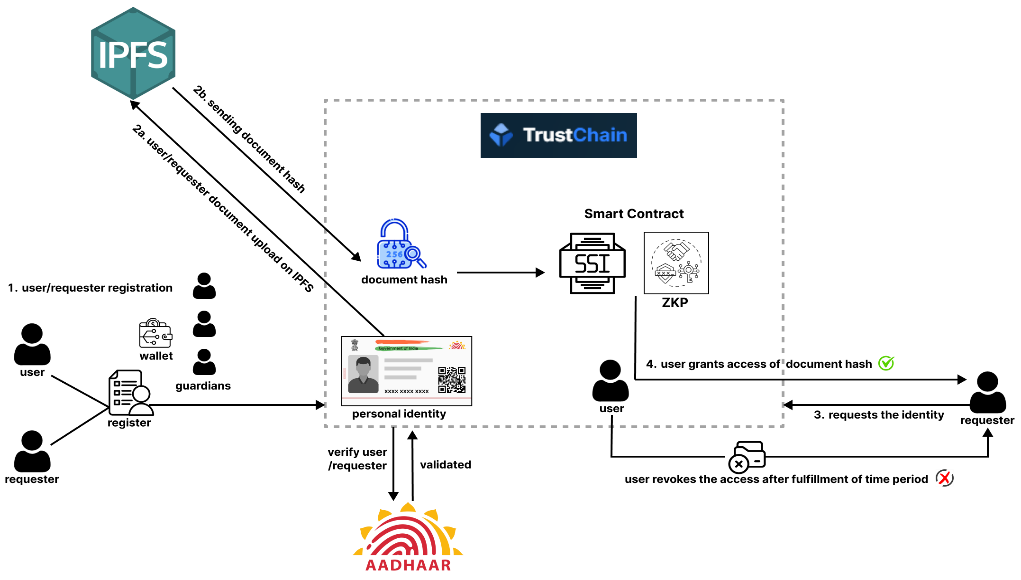
\includegraphics[width=1\textwidth]{Chapter1/trustchain_architecture.png} % Adjust the width as needed
    \caption{TrustChain Framework Architecture}
    \label{f1} % Optional: for referencing the figure in your document
\end{figure}


TrustChain framework is developed as a fully user centric identity life cycle that is privacy, control and secure verification oriented. The architecture allows identity not to be revealed in crude form but instead facilitates the verification to occur effectively. This is a system that is based on the decentralized technologies which use the combination of blockchain and IPFS, Self Sovereign Identity and Zero Knowledge Proofs. It brings in an ordered sequence of activities, starting with safe onboarding, then credential storage, hashing, verification and access control. There is an attention to each stage where it is designed to remove the redundant data sharing with integrity and trust. The architecture also makes sure that the users are in complete control of their identity during the process. The framework solves the major problems of misuse of data and unauthorized exposure of data in current systems by moving away the traditional document based verification into the proof based verification. It also develops a generalized flow which can be embraced in various fields. The modular design enables an easy extension and upgrade in the future. The system design will have the ability to be compatible with the emerging digital identity standards. This renders the architecture to be scalable and suitable to long term use.

The system starts by having a user registration process which is non redirectional making the on boarding process smooth. Users are expected to put in three guardian wallet addresses during registration that are used as recovery agents. Such guardians are significant in the recovery of the accounts in case they get lost. This ensures that it is not highly reliant on centralized recovery systems. It also enhances trust because recovery is spread among the entities that are trusted. The onboarding is maintained simple so as to make it easy to use. This enhances its adoption by non technical users also.


After the registration process, the system first does initial verification and safely creates a master private key to the user. This key is shared with the individual and is the central control and authentication mechanism among the platform. The key will make sure that verification actions can only be taken by the owner. Key handling practices need to be properly applied to ensure security. This enhances the authentication system of the system. It also complies with the decentralized identity ownership principles.

Following the onboarding, the users post their government identity documents to the platform. They are stored in IPFS as PINATA that provides a decentralized and safe storage. IPFS assigns a content identifier to every document that serves as the foundation of additional cryptographic processes in the system. This eliminates the necessity to have centralized stores. It enhances fault tolerance and availability too. Information in the form of documents cannot be easily accessed by mere queries. This guarantees an added level of security.

To increase the level of security, the IPFS generated hash is subjected to another round of hashing with keccak256. This hash is then hashed again, to make sure it is irreversible. This hybrid hash method ensures that there is no chance of restoring the original document and at the same time be able to check the integrity. It enhances opposition to brute force attacks. The stacked hashing structure makes life more difficult on the part of attackers. This guarantees security as opposed to single hash systems. It is also efficient in the verification operations.

The identity verification is developed based on the principles of Self Sovereign Identity where a user has control over his or her data. There is limited information that is shared like name, email and date of birth. Checking is done through the Zero Knowledge Proofs that verify authenticity without exposing sensitive information. This will minimize unnecessary exposure of data when it is verified. It provides adherence to privacy oriented needs. Access duration can be defined depending on the need of the users. This provides full freedom in the use of identities.

ZK STARK is utilized when generating proofs since it is based on hash functions and does not require the trusted setup. It makes it more resistant to attacks, e.g. replay or inference attempts. The verification process is used to compare the calculated hashes with the stored values on chain to confirm the authenticity of the identity. This enhances trust on the verification outcomes. It minimizes the need to rely on third party validation systems. The generation of proof can be done in adversarial conditions as well without being compromised. This renders the system strong to be used in the real world.

The entire access control mechanism is controlled by smart contracts deployed with Solidity on the OP Sepolia Testnet. They give requesters merely demonstrations of validity as opposed to real documents. Users have the permission to give, deny or take back access anytime and everything is documented on the blockchain ensuring transparency, security and applicability in real world domains. This leaves a permanent chronicle of all the activities. It makes sure that there is accountability of each access request. The system does not deal with any form of financial transactions to ensure that it does not lose sight of identity checking. This makes the architecture very straightforward and functional.




\rule{0.49\textwidth}{0.75pt} $_{\bigcirc}$ \rule{0.49\textwidth}{0.75pt}\\

\clearpage 
\chapter[Project Management]{Project Management}{Project Management}\label{projm}


\rule{0.49\textwidth}{0.75pt} $_{\bigcirc}$ \rule{0.49\textwidth}{0.75pt}\\





\section{Feasibility Study}

\subsection{Technical Feasibility}
TrustChain has a high technical feasibility with well established and widely adopted technologies used in the frontend and backend layers. The frontend will be constructed in HTML5, CSS3 and React.js which will provide a responsive and easy to use interface to register, access and manage the dashboard. It can be integrated with Web3.js or Ethers.js to allow the user interface to interact with blockchain smart contracts easily. This will provide a smooth communication and real time updates of identity verification workflows within the system.

On the backend, there is the use of Node.js and Express.js that deal with the server side operations, API management and communication between the various parts of the system. IPFS integration (Pinata) is a way to achieve the decentralization of identity documents storage which enhances their availability and fault tolerance. Decentralized identifiers, access control and verification logic are implemented in Solidity based smart contracts running on the blockchain layer with Ethereum. Metamask and WalletConnect are embedded tools to facilitate secure wallet authentication and to interact with the blockchain network effectively.

The system also includes cutting edge cryptographic and identity systems like Self Sovereign Identity and ZK STARK based verification. These technologies provide the identity validation to be done without exposing sensitive information and retain the integrity of proofs with the help of KECCAK 256 hashing. This combination is what results in the system being technically sound and in line with the current standards of security.

Design wise, TrustChain adheres to the human centered design principles to make it user-friendly and easily accessible. The user flow remains minimal and has a straightforward onboarding, upload and access document management. This makes it possible to have even the non technical users to interact with the system effectively without having to jeopardize security or functionality of the system. The interface is to be as user friendly as possible and yet easy to understand every step of the process. This enhances the general usability and promotes usage by a broader group of users.
\subsection{Operational Feasibility}

The operational feasibility of TrustChain revolves around how it is able to operate in real world identity verification situations. The system will act in tandem with the other pre-existing systems like the government systems and telecommunication systems. It will act as a verification layer of middle ground to allow smooth adoption and not necessitate a total overhaul of existing systems and workflows. It minimizes reliance on manual verification processes within the departments. This aids in quick processing and delivery of services. The system can be incorporated without impairing the current workflows.

The interaction process is easy and arranged to ensure users can register, upload documents and access them without being complicated. Features such as guardian based recovery and controlled access ensure reliability in case of user errors or access issues. The system reduces repetition of data entry that enhances efficiency and minimizes overhead costs of operation by the users and requesting entities. The users can simply know and manage their data sharing preferences. This enhances confidence and minimizes misunderstandings when verifying. The platform provides uniform experience to various uses.

Institutionally, TrustChain lessens the burden of managing sensitive identities information through offering proof based verification. Raw documents are not sent to organizations but only validation results making it easier to comply and less risky. Smart contracts provide automation of access control and keep transparent a log of all activities on the blockchain. It also minimizes the chances of data duplication and inconsistencies. The automation of logs enhances operations traceability and auditability. This enhances accountability in organizations that use the system.

The system is also scalable in terms of operations, taking advantage of the use of decentralized storage and blockchain infrastructure. It provides uniform performance without any centralized bottlenecks. This renders TrustChain to be applicable in the implementation in various industries that need secure and effective identity checking. Its decentralized structure allows high availability when it is being used to the fullest. It mitigates risks that are caused by centralization system failures. This ensures uninterrupted access and reliable verification services.
\subsection{Economic Feasibility}
Decentralized infrastructure and use of open source technologies can support the economic viability of TrustChain. It eliminates the cost of having costly centralized storage and data management systems. This reduces first development cost and guarantees scalability and durability.

The system lowers the cost of operation by decreasing the number of times of identity verification and the number of times of handling sensitive documents manually. Organizations do not have to invest much in secure storage infrastructure because data is stored in IPFS. Verification and access control are automated by the use of blockchain smart contracts, cutting down on administrative overhead. Moreover, integration with the existing systems will not incur the expense of replacement of the entire infrastructure and the solution is thus cost effective to adopt.

In the long term, TrustChain will help to minimize financial losses related to identity fraud and data breaches. It reduces the risks that identity data can be misused by making sure that the verification is secure and privacy preserving. The scalable architecture is also economically viable as it minimizes maintenance costs in the long run and can be deployed in large scalable manner across sectors.


\section{Project Management}
\subsection{Timeline Chart}
Below are the key milestones for the TrustChain project, along with an estimated timeline based on standard software development cycles and the methodologies described in our research paper.

\begin{table}[h!]
\centering
\begin{tabular}{|p{4cm}|p{7cm}|p{4cm}|}
\hline
\textbf{Milestone} & \textbf{Description} & \textbf{Estimated Completion Date} \\
\hline
Project Initiation \& Planning & Define project scope, create team, collect requirements & August, 2025 \\
\hline
System Design \& Architecture & Design system layers, identity flow and identity access control & September, 2025 \\
\hline
Frontend \& Backend Development & Develop user interface, backend APIs and integrate wallet authentication & November, 2025 \\
\hline
IPFS \& Hashing Implementation & Deploy a multi layer hashing and decentralized storage & December, 2025 \\
\hline
Blockchain \& Contract Development & Write smart contracts to check identity and access control & January, 2026 \\
\hline
Testing \& Validation & Conduct functional, security and performance testing of the system & February, 2026 \\
\hline
User Feedback \& Iteration & Collect feedback and improve usability and system flow & March, 2026 \\
\hline
Deployment \& Integration & Deploy system and test integration to real world use cases & March, 2026 \\
\hline
Final Review \& Documentation & Complete documentation and finalize project report & April, 2026 \\
\hline
Conference Presentation & Write research paper and present at ICTIS conference. & April, 2026 \\
\hline
\end{tabular}
\caption{TrustChain Project Milestones and Timeline}
\end{table}

\\ 


\section{Project Resources}

\subsection{Hardware Requirements}
TrustChain hardware requirements are specified by the necessity to develop, deploy and ensure identity verification in case of different user roles like developers, users and requesting entities. These requirements guarantee the best performance, system responsiveness and safe use of the platform.

1. Development and Hosting Server Requirements
Processor: Intel Core i7 (or equivalent AMD Ryzen 7) – 8th Gen or higher

RAM: Minimum 16 GB (Recommended: 32 GB for for handling blockchain and cryptographic operations)

Storage: 1 TB SSD (Solid State Drive) for faster data access and efficient IPFS integration

GPU (Optional): Not mandatory, as no heavy machine learning training is involved

Internet: High speed broadband with upload/download speeds of at least 100 Mbps

Power Backup: UPS or generator backup to ensure continuous uptime during outages

2. Client Side (Users and Requesters)
Processor: Intel Core i3 or higher

RAM: Minimum 4 GB (Recommended: 8 GB for smoother performance)

Storage: 250 GB HDD or SSD

Compatibility with Devices: compatible with laptops, smartphones, tablets and desktops.

Display: Minimum resolution of 1366 x 768 pixels

Internet: Stable internet connection with 10 Mbps speed for seamless interaction and verification processes



\subsection{Software Requirements}

1. Operating System\\
Development Environment:
Windows 10/11 (best used when setting up blockchain nodes), macOS (use cross platform testing)
Client Environment (User Side):
Windows 10/11, Android 8.0+, iOS 13+, or any other operating system with a current web browser.

2. Frontend Technologies\\
Language: HTML5, CSS3, JavaScript
Framework: React.js (v18) – to create responsive and dynamic user interfaces.
Styling Libraries: Tailwind CSS or Bootstrap (to have a consistent UI design.)

3. Backend Technologies\\
Runtime Environment: Node.js (v16 or above) to scale on server side.
Framework: Express.js (v4.17.1) to route HTTP requests and API.
Decentralized Storage: IPFS with Pinata integration for storing identity documents.

4. Blockchain Layer\\
Platform: Ethereum Network ( OP Sepolia Testnet to deploy and test)
Smart Contract Language: Solidity to verify identity and access control logic.
Wallet Integration: Metamask or WalletConnect to sign a transaction and authenticate.

5. Identity Layer \& Cryptography\\
Framework: Self Sovereign Identity to decentralized identifiers and verifiable credentials.
Mechanism Proof: ZK STARK privacy preserving identity verification.
Hashing Algorithm: KECCAK 256 to verify the integrity of data and validate proofs.

6. Development Deployment Tools\\
Version Control: Git with GitHub integration.
Package Managers: npm to deal with project dependencies.
IDE or Text Editors: Visual Studio Code or any development environment of choice.



\section{Project Estimation}

\subsection{COCOMO Estimation Model}
In order to determine the development effort of TrustChain, the Basic COCOMO Model is used under Semi Detached category since the project contains moderate complexity with the integration of blockchain, cryptographic operations and a team with mixed levels.
\\
\\
Estimated Size: 14,000 lines of code (14 KLOC)\\
Effort (E): $E = 3.0 \times (14)^{1.12} \approx 57 \text{ person-months}$\\
Development Time (D): $D = 2.5 \times (57)^{0.35} \approx 9 \text{ months}$\\
Team Size (P): $P = \frac{57}{9} \approx 6 \text{ members}$

\begin{table}[h!]
\centering
\begin{tabular}{|l|l|}
\hline
\textbf{Parameter}        & \textbf{Value}       \\
\hline
LOC                      & 14,000             \\
Effort                   & \textasciitilde57 PM    \\
Development Time         & \textasciitilde9 months \\
Team Size                & \textasciitilde6 members \\
\hline
\end{tabular}
\caption{Project Parameters}
\label{tab:project_parameters}
\end{table}


\subsection{Function Point Analysis}
Function Point Analysis (FPA) estimates the size and effort of TrustChain by evaluating its functional components such as user inputs, outputs, storage and blockchain interactions. The method does not depend on the programming language and is oriented towards the functionality of the system.

1. Component Breakdown

\begin{table}[h!]
\centering
\begin{tabular}{|l|c|l|c|c|}
\hline
\textbf{Component}                                   & \textbf{Count} & \textbf{Complexity} & \textbf{Weight} & \textbf{Total FP} \\
\hline
External Inputs (registration, upload, access)              & 6     & Medium     & 4      & 24       \\
External Outputs (verification result, proof)          & 4     & Medium     & 5      & 20       \\
User Inquiries (status check, access logs)             & 3     & Simple     & 3      & 9       \\
Internal Logical Files (user data, hashes) & 4     & Medium     & 7      & 28       \\
External Interface Files (IPFS, APIs)             & 3     & Medium     & 7      & 21       \\
\hline
\textbf{Unadjusted Function Points}              &       &            &        & \textbf{102}  \\
\hline
\end{tabular}
\caption{Function Points Calculation}
\label{tab:function_points}
\end{table}

2. Complexity Adjustment
Based on the system features like security, distributed processing, cryptographic computation and integration complexity, a Complexity Adjustment Factor (CAF) of 1.08 is used.
\\
Adjusted Function Points (AFP): $AFP = 102 \times 1.08 \approx 110$\\

3. Effort Estimation
With an average of 10 hours per function point:

Total Effort = 110 × 10 = 1,100 hours\\

A full-time (90 hours/month/person) 3-person team:

Time: $T = \frac{1100}{3 \times 90} \approx 4 \text{ months}$

\rule{0.49\textwidth}{0.75pt} $_{\bigcirc}$ \rule{0.49\textwidth}{0.75pt}\\

\clearpage 

\chapter[System Design]{System Design}{System Design}\label{sd}

\noindent
\rule{0.49\textwidth}{0.75pt} $_{\bigcirc}$ \rule{0.49\textwidth}{0.75pt}\\

\section{Design Diagrams}

\subsection{Data Flow Diagram}
 \begin{figure}[h!]
     \centering
     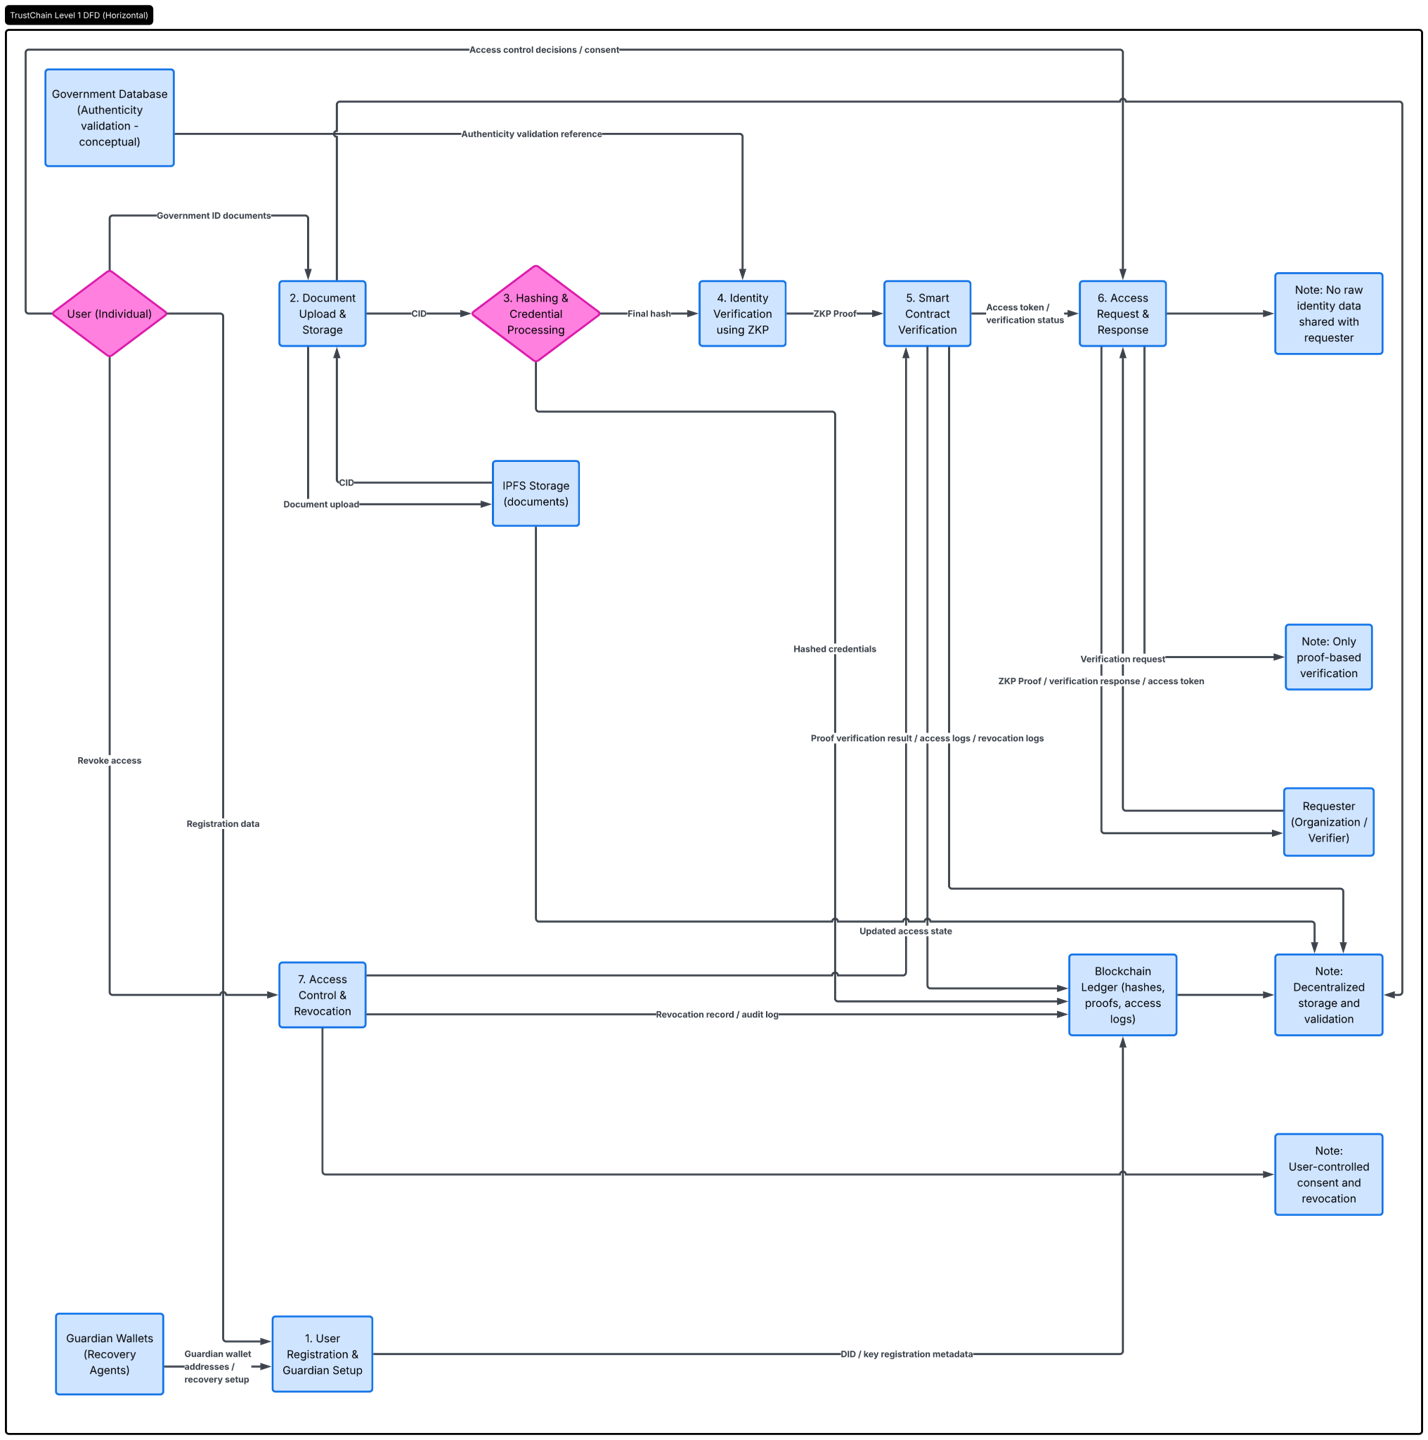
\includegraphics[width=1\textwidth]{Chapter1/DFD.png} % Adjust the width as needed
     \caption{Data Flow Diagram}
     \label{f1} 
\end{figure}
Data Flow Diagram of TrustChain is the general flow of data in the system showing the processing of the identity information safely without exposing it. In the diagram, interaction is shown between user entities and the internal processes of the system and the decentralized elements of IPFS and blockchain. It distinctly outlines the movement of data (between registration and verification) by maintaining privacy control and integrity at all levels of the system design and implementation. This framework can be used to comprehend secure communication and system dependencies.

The flow chart starts with the registration of users and guardians in which members input necessary information and allocate recovery wallets. Such wallets serve as trustworthy sources that allow the restoration of accounts and keep control in the event of loss of access. The information on registration is fed into the system that triggers the creation of identity and its connection to decentralized identifiers and cryptography keys that guarantee ownership and secure authentication throughout the platform. It also lays the foundation of initial trust relations needed in subsequent verification processes in system flow.

Users register with their identity documents that are kept on IPFS with decentralized storage system. The system creates a content identifier of every document and it is processed with multi layer hashing with keccak based operation. This provides assurance that no unprocessed document is ever exposed and integrity is maintained and allows the secure work process across constituents. The hashes generated are processed to derive proofs and check that they are consistent.

Then the diagram shows how identity verification can be done with Zero Knowledge Proofs where hashed credentials are verified without disclosing sensitive information. The mechanism of ZK STARK guarantees cryptographic security and avoids trusted setup. These evidences are then provided to smart contracts deployed on the blockchain that execute verification logic and impose role based access control. The blockchain stores hashes proofs and access logs that guarantee the transparency immutability and auditability of any operation, conducted in the system. This measure enhances inter-party trust and ensures high- privacy standards throughout interactions.

Lastly the access request and response process enables the requesters to authenticate identity with proof based validation as opposed to accessing real documents. Users are in full control of their data by giving or withdrawing permissions anytime during interactions with smart contracts. Every activity is documented on the blockchain which guarantees irreversible records and responsibility. The diagram focuses on decentralized storage user permission and secure validation that ensure the system is scalable and reliable to be implemented in the real world identity verification applications. It also emphasizes connectivity between frontend backend and blockchain layers that guarantee a smooth flow of data and efficiency of operation.





\subsection{Use Case Diagram}


\begin{figure}[h!]
    \centering
    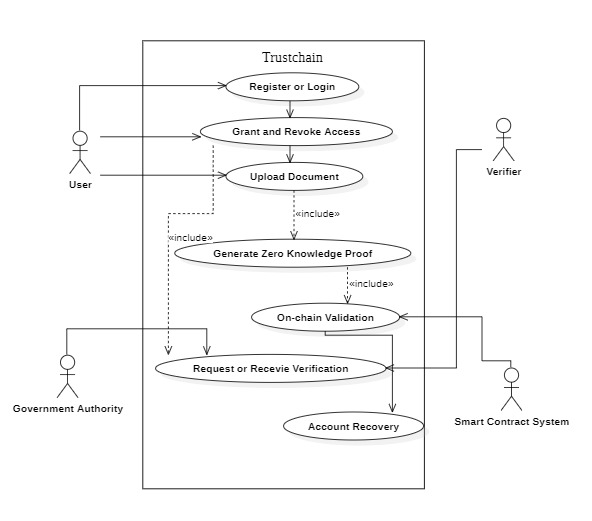
\includegraphics[width=1\textwidth]{Chapter1/use_case_new.jpeg} % Adjust the width as needed
    \caption{Use Case Diagram }
    \label{f1} % Optional: for referencing the figure in your document
\end{figure}
The Use Case Diagram of TrustChain shows how the various actors and the system interact with each other, in this case emphasizing the manner in which identity verification can be carried out without exposing sensitive data. It emphasizes the user centric control, secure identification and decentralized verification protocol. The diagram also clearly illustrates the boundaries of the systems, and the participation of each actor in the life cycle of identity within the platform.

The key players of the system are the User, Requester and Guardian Wallets. The User communicates with the system to register, upload and get access to documents. The Requester sends verification requests to verify identity without access to raw documents. Guardian Wallets are recovery agents, which guarantee safe account recovery. All the actors have well defined roles that aid in ensuring system security, reliability and user control during identity verification process.

The user can get started by registering on the site and creating guardian wallets to recover them. Once onboarded successfully the user uploads identity documents once. Such documents are safely stored and manipulated in the system to create verifiable credentials and hashed representations to be verified further.

The requester engages the system by making a verification request. The system does not handle real identity documents but instead does the request based on cryptographic proofs. The user is alerted and he can approve or reject. This guarantees verification is carried out at the consent of the user and the full privacy of sensitive information.

It has several processes that are done internally such as hashing and Zero Knowledge Proof generation and validation of smart contracts. All these mechanisms combine and authenticate identity without exposing personal information. An access control is implemented with the help of smart contracts on the blockchain where permissions can be granted and denied. All the interactions are documented to maintain transparency and traceability as well as to secure and efficient verification workflows.

Altogether, the Use Case Diagram focuses on a privacy first design, in which the users will be in charge of their identity information. It shows how TrustChain is used to substitute the traditional document sharing with the use of proof based validation. Secure interactions among actors as well as system components to guarantee a scalable, reliable and user friendly identity verification solution are also emphasized in the diagram.


\subsection{Data Structure Design and Smart Contract}
The TrustChain Smart Contract and Data Structure Design eliminates the necessity of a conventional database schema and uses the blockchain and decentralized storage systems. Rather than having centralized systems holding raw identity data, the architecture concentrates on having structured references like hashes, proofs and access states. This will make sure that no sensitive information is directly exposed, at the same time making it possible to effectively verify identity. The architecture is a hybrid in that, critical verification information is stored on chain, and real documents are off chain in IPFS.

Smart contracts serve as the first layer in the system of data management. They take care of storing hashed credentials, decentralized identifiers and upholding access control logic. Every user is linked to a distinctive identity framework comprising of hashed document references and permission states. Verification requests, responses and revocation actions are also documented in the contracts. This organised method also guarantees immutability, traceability and safe management of identity related processes without the use of central databases.

Integration of IPFS compliments blockchain as it deals with storage of documents in a decentralized fashion. The smart contracts only contain links to content identifiers and hashes derived, providing integrity without revealing raw content. Access logs and proof validation records that make data structure also allow auditability. This architecture guarantees scalability, privacy and effective data processing.


\rule{0.49\textwidth}{0.75pt} $_{\bigcirc}$ \rule{0.49\textwidth}{0.75pt}\\

\clearpage 

\chapter[Implementation]{Implementation}{Implementation}\label{im}

\noindent
\rule{0.49\textwidth}{0.75pt} $_{\bigcirc}$ \rule{0.49\textwidth}{0.75pt}\\


\section{Implementation Tools, Data Handling Approach and System Limitations}
TrustChain implementation aims at data handling, with a focus on secure data handling as opposed to conventional data collection. React based forms are used to gather user inputs in the registration, guardian set-up and uploading of documents. The backend is done in Node.js and Express.js APIs. The upload of files is processed and sent to IPFS through Pinata that ensures decentralization. The Web3.js or Ethers.js is utilized to interact with blockchain and to enable the frontend to interact with the smart contracts to verify identity creation and access control. The frontend also takes care of the correct input validation prior to transmitting data to the backend services. Metamask, which uses wallet based authentication, enhances security and user ownership. It will not store sensitive data in the centralized servers. The API communication is designed such that it is consistent and reliable. This will provide ease of interaction among all layers of the architecture.

The system does not follow a conventional sample size approach as it is not data driven but identity driven. The platform does not deal with huge datasets but processes single identity records in real-time. Documents are uploaded by each user and unique hashed credentials are generated, used to verify the user again. Hashing mechanisms and decentralized storage are used to optimize data handling and reduce redundancy and enhance efficiency. The verification requests are dynamically executed in accordance with user permission and consent within smart contracts. The system has been planned to support multiple verification requests concurrently without any impact on the system. Processing with hash based processing provides the transfer of very little data between components. This save bandwidth and enhances efficiency in response. The verifications are independent to each other and this enhances scalability of operations. The architecture will be capable of extension in the future to accommodate more users.

Limitations:
The system implementation has certain constraints. The dependency on user supplied documents creates dependency on preliminary authenticity checks which are conceptually connected to government databases. Blockchain transaction and wallet interaction error handling can be complex to the non technical user. Also, the latency of networks in IPFS and blockchain activities can influence the response time. Large scale deployments can also be problematic due to the lack of rate limiting and advanced monitoring mechanisms and will have to be further optimized. In certain instances, wallet management may pose usability issues because users are dependent on it. Without appropriate recovery arrangements, loss of personal keys can result in difficulties in accessing them. It still remains in conceptual stage as it has to be integrated with other external systems such as government databases. Upgrades of smart contracts are tricky when they are deployed and need to be planned. These aspects underline the future areas of the improvement and development.

\section{Identity Data Structure and Cryptographic Components Description}
User Identity Data:

User related information like wallet address, decentralized identifier and linked guardian wallets. It also has fewer personal attributes such as a name, email and date of birth that are controlled to verify.
Applications: It is applied in authentication, ownership of identities and in controlling access rights in the system.

Credential Data:

Contains uploaded government identity documents on IPFS and the content identifiers generated. These credentials are never kept in the raw form on chain and are connected by hashed references.
Usage: It is applied to producing verifiable proofs, and retaining integrity of identity without revealing real documents.

Hash Data:

Represents multi layer hashed values of IPFS content identifiers using KECCAK 256 and secondary hashing. These hashes are secure representations of original documents.
Applications: The identity can be verified and compared during the process of verifying proof.



\section{Cryptographic Data Preparation and Processing}

The TrustChain system substitutes the traditional methods of preprocessing with cryptography processing method aimed at securing identity data prior to the verification process. After uploading identity documents, the system will directly turn them into secure representations in IPFS that creates a unique content identifier. This identifier gets hashed using KECCAK 256 and another hashing to make sure that it is irreversible. This stage of preparation is aimed at making sure that there is no raw data stored or relayed in the system. The resultant hashes are then formatted in such a way that they can be fed into Zero Knowledge Proof generation where ZK STARK algorithms are run over the hashed values to give verifiable proofs. With this method, there is no data cleaning or transformation like in the traditional systems. Rather, it is about providing the integrity of data, privacy and consistency of decentralized components. The ready cryptographic messages are then utilized throughout the verification lifecycle allowing the safe comparison, validation and access control without the disclosure of sensitive identity information.

\section{Description of Algorithms (Modular)}

Identity Check and Access Control:\\
Algorithm: ZK STARK (Zero Knowledge Scalable Transparent Argument of Knowledge) privacy preserving identity verification.\\
Usage: Checks user identity, creating cryptographic proofs of hashed credentials without disclosing any sensitive data. It assures the user that he or she is authentic and keeps all the data confidential throughout verification requests.\\

Hashing and Data Integrity:\\
Algorithm: KECCAK 256 multi layer with hashing.\\
Usage: Convert identifiers of IPFS generated content to secure irreversible hashes. These hashes serve as distinct identities of identity documents and are compared and verified without revealing raw data.\\

Decentralized Storage:\\
Algorithms: IPFS content addressing scheme.\\
Usage: Stores user uploaded identity-documents in a decentralized format and obtains a unique identifier of a content in a file. This guarantees high availability, fault tolerance and avoids reliance on centralized storage systems.\\

Smart Contract Verification:\\
Algorithm: Open source Ethereum Solidity based smart contract logic.\\
Usage: Runs the verification rules, handles the decentralized identifiers and implements the role based access control. It authenticates evidence and records of access requests, approvals and revocations that cannot be altered.\\

Wallet Based Authentication:\\
Algorithm: Public and Private Key Cryptography.\\
Usage: Signs wallets with Metamask or WalletConnect to authenticate users. It makes sure that the actions are initiated within the system by the rightful owner of the identity.\\

Access Control and Revocation:\\
Algorithm: Role Based Access Control based on smart contracts.\\
Usage: Controls permission states, period of access and revocation. It enables users to issue or revoke access on a dynamic basis with all the actions being logged transparently on the blockchain.\\

\section{Description of Tools for Implementation}

VS Code Visual Studio code:
Description: A source code editor created by Microsoft, which is light in weight but powerful.
Usage: Writing, debugging and administration of the frontend, back-end and smart contract code, offers an efficient development experience with blockchain and web technology extensions.

Git:
Description: A distributed version control system to track source code changes.
Usage: Controls versioning of an entire system during development, facilitating effective collaboration, tracking of code and retracting changes during various phases of the project.

GitHub:
Description: A web based platform for hosting and collaborating on Git repositories.
Usage: Manages the TrustChain project repository where people can collaborate, manage versions, track issues and maintain the project history with adequate documentation.

Postman:
Description: An API development and testing tool.
Usage: Tests and debugs API endpoints, ensuring they function correctly and meet the application's requirements.

MetaMask:
Description: A blockchain interaction and cryptocurrency wallet. Applications: Authenticate wallets, sign transactions and allow users to safely communicate with Ethereum smart contracts when verifying their identity and controlling access in an identity verification and access control operation.


\section{Interface Design}
The design of the platform interface of TrustChain is centered on simplicity, clarity and control by the user with secure interactions. The React.js frontend offers a simplistic dashboard to register, upload and access documents. Verification requests can be easily viewed, permission and track activity can be granted or revoked. An integration of wallets means that authentication is provided without involving complicated procedures. The system is designed along the human centered concepts and thus the system is reachable by both the technical and non technical users without compromising on efficiency and security during the flow of interactions.


\rule{0.49\textwidth}{0.75pt} $_{\bigcirc}$ \rule{0.49\textwidth}{0.75pt}\\

\clearpage 

\chapter[Testing]{Testing}{Testing}\label{Test}
\noindent
\rule{0.49\textwidth}{0.75pt} $_{\bigcirc}$ \rule{0.49\textwidth}{0.75pt}\\
In Trustchain testing is essential to making sure that the system works safely, reliably and as expected by all parts. Given the sensitivity of identity verification by the platform, extensive testing is necessary to confirm data integrity, access control mechanisms and general system behavior. The aim of the testing process is to detect problems in the initial stages and verify that each module is functioning properly in various conditions.

Tests are done at various levels such as frontend, backend and blockchain interactions. Functional testing is conducted to test user flows like registration, document upload, verification requests and access control. Integration testing is the method that promotes the seamless interaction of the parts, such as React frontend, Node.js backend, IPFS storage and smart contracts that are stored on the blockchain.

Automated testing of user interface workflows, end to end scenarios are done through the katalon studio. It assists in authentication of user behaviors, form submissions and system replies. Postman is widely applicable in API testing where API endpoints are given tests to determine their ability to handle requests accurately with errors and thus reliably communicate between the components of the system.

As well, there is testing of cryptographic algorithms like hashing and proof verification. Testing of smart contracts is done to verify proper implementation of access control and verification logic. This holistic solution assures TrustChain of security, performance and reliability in real world deployment scenarios.
\\
\noindent

\section{Test Cases}



\renewcommand{\arraystretch}{1.1}
\begin{center}
\textbf{Test Cases Overview}
\end{center}

\begin{longtable}{|p{1.1cm}|p{2cm}|p{2.5cm}|p{3cm}|p{3cm}|}
\hline
\textbf{Test Case ID} & \textbf{Feature} & \textbf{Test Scenario} & \textbf{Test Steps} & \textbf{Expected Result} \\
\hline
\endfirsthead

\hline
\textbf{Test Case ID} & \textbf{Feature} & \textbf{Test Scenario} & \textbf{Test Steps} & \textbf{Expected Result} \\
\hline
\endhead

\hline \multicolumn{5}{r}{\emph{Continued on next page}} \\
\endfoot

\hline
\endlastfoot

TC01 & Wallet Connection & Validate wallet connection and role selection & 1. Click connect wallet 2. Select role & Wallet connects and role selected. \\
\hline
TC02 & User Registration & Validate user registration with details & 1. Enter name email guardians 2. Submit form & User registered successfully. \\
\hline
TC03 & User Login & Validate login using wallet authentication & 1. Click login 2. Authenticate wallet & User logged in dashboard displayed. \\
\hline
TC04 & Add Credential & Validate adding new credential & 1. Enter details 2. Upload document & Credential added successfully. \\
\hline
TC05 & IPFS Storage & Validate document storage on IPFS & 1. Upload document 2. Submit data & Document stored hash generated. \\
\hline
TC06 & Hash Generation & Validate credential hash generation & 1. Upload credential 2. Process hashing & Secure hash generated successfully. \\
\hline
TC07 & View Credentials & Validate viewing stored credentials & 1. Open credentials 2. View list & All credentials displayed correctly. \\
\hline
TC08 & Request Handling & Validate receiving verification requests & 1. Open sharing tab 2. View requests & Requester and hashes displayed. \\
\hline
TC09 & Grant Access & Validate granting access to hash & 1. Select request 2. Click grant & Access granted successfully recorded. \\
\hline
TC10 & Revoke Access & Validate revoking granted access & 1. Select request 2. Click revoke & Access revoked successfully updated. \\
\hline
TC11 & Role Selection & Validate switching user roles & 1. Select role 2. Confirm action & Interface updates based on role. \\
\hline
TC12 & Data Privacy & Validate no raw document exposure & 1. Share credential 2. Verify output & Only hash shared not document. \\
\hline
TC13 & Smart Contract & Validate blockchain transaction execution & 1. Perform action 2. Confirm transaction & Transaction recorded on blockchain. \\
\hline
\end{longtable}

\rule{0.49\textwidth}{0.75pt} $_{\bigcirc}$ \rule{0.49\textwidth}{0.75pt}\\




\clearpage 
\chapter[Results and Discussions]{Results and Discussions}{Results and Discussions}\label{res}
The findings indicate the realistic application of the TrustChain model as a working web based decentralized identity verification system. The interfaces put in place en-sure validation of controlled access, privacy preserving verification and on-chain auditability of actual user and institutional interactions. The dashboard enables registered institutions to find individuals and make credential access requests. The organization will be able to seek verification without looking at the raw identity documents, which will enforce a least privilege access rule. This screen is used to capture the user approving the access by providing the credential hash only. Authentication of identity is done by cryptographic validation, and not by document disclosure. Successful verification is displayed in this interface in which access is granted and validated. The institution is presented with proof of originality without the access to personal identity information. This is the last perspective in which institutions can check the verification status of an individual. The outcome warrants identity validity and privacy and continues access control that is revocable. This illustrates the usefulness of a proof based verification model in the real world. The system is able to remove needless data exposure and at the same time retain trust between entities. It also emphasizes the role of user controlled consent in the process of identity sharing. The findings verify that decentralized strategies may be beneficial in terms of security and transparency. This enhances the possibility of integration with the current digital identity ecosystems. TrustChain is an overall viable and scalable solution to privacy oriented identity verification.

\section{Outputs}
\begin{figure}[h!]
    \centering
    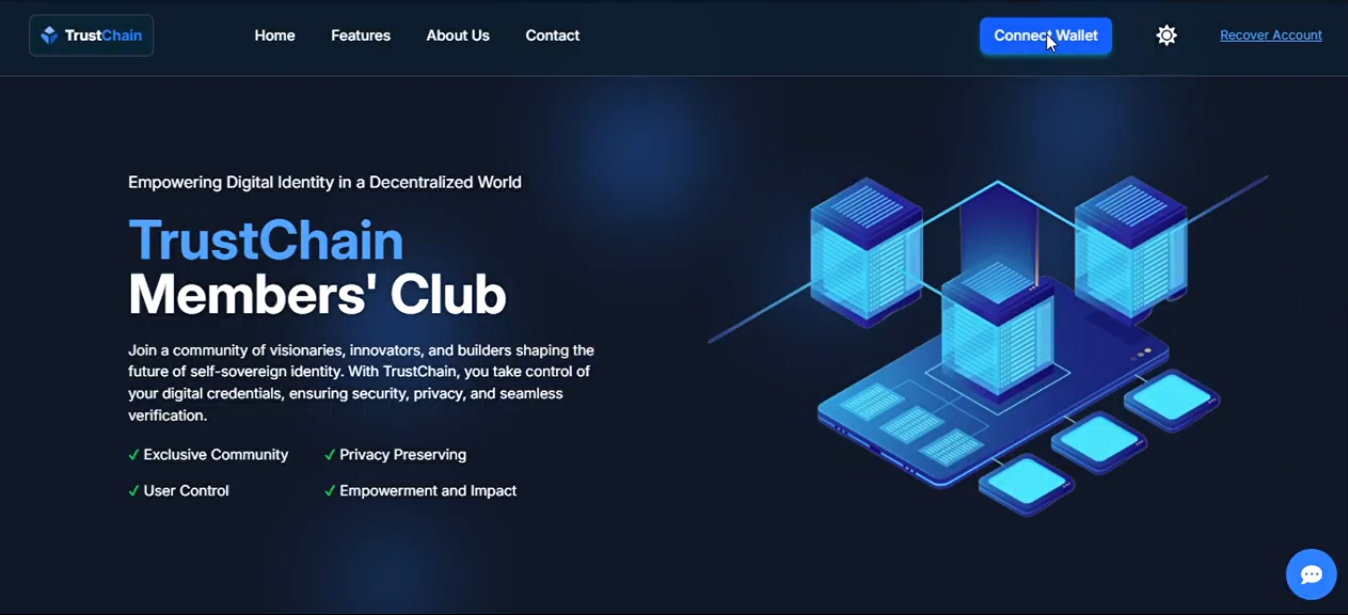
\includegraphics[width=0.8\textwidth]{Chapter1/dashboard.png} % Adjust the width as needed
    \caption{TrustChain Dashboard}
    \label{f1} % Optional: for referencing the figure in your document
\end{figure}

\begin{figure}[h!]
    \centering
    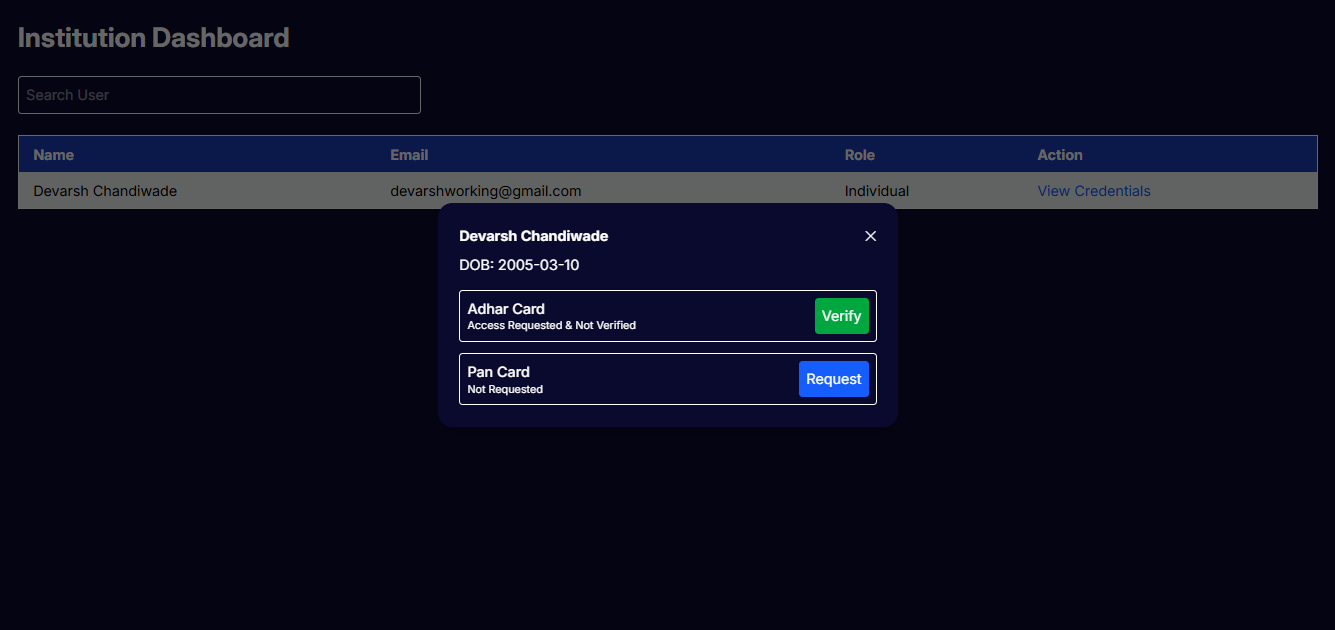
\includegraphics[width=0.8\textwidth]{Chapter1/ss2.png} % Adjust the width as needed
    \caption{Institution Dashboard for Credential Request}
    \label{f1} % Optional: for referencing the figure in your document
\end{figure}

\begin{figure}[h!]
    \centering
    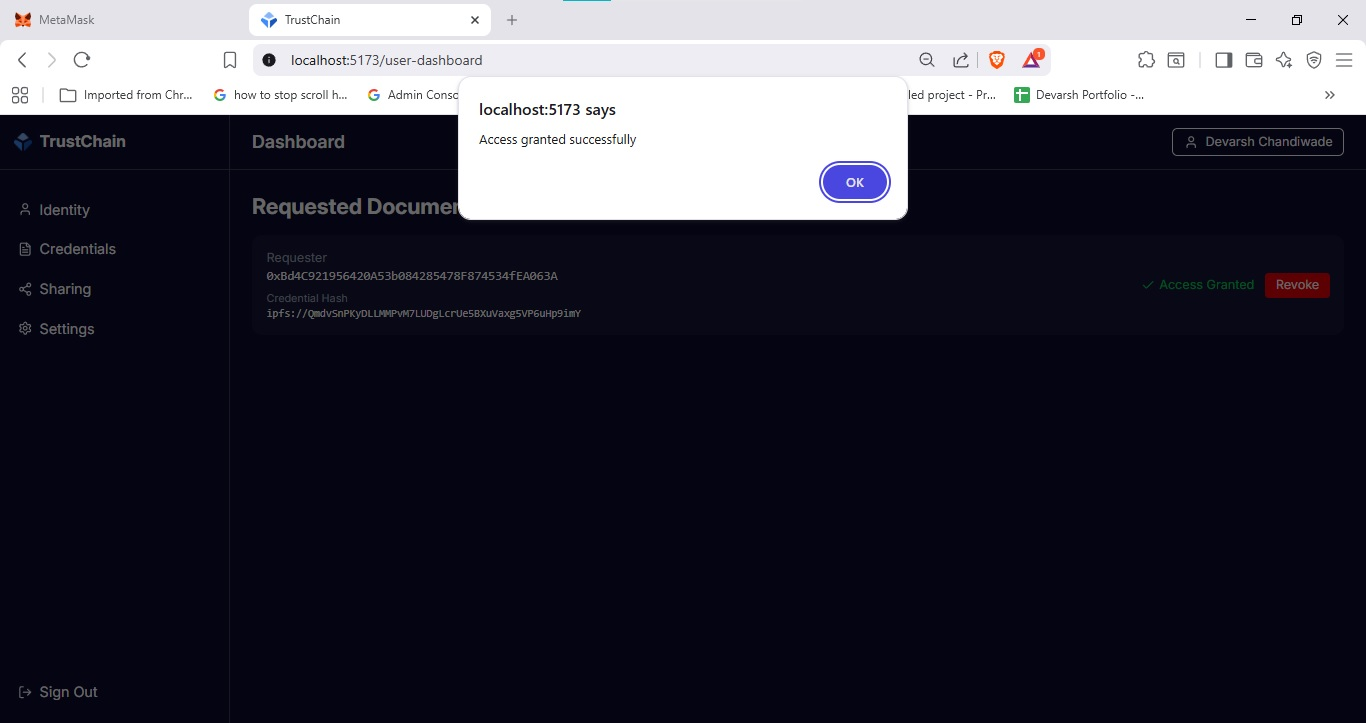
\includegraphics[width=0.8\textwidth]{Chapter1/ss4.jpeg} % Adjust the width as needed
    \caption{Individual Granting Credential Hash Access}
    \label{f1} % Optional: for referencing the figure in your document
\end{figure}

\begin{figure}[h!]
    \centering
    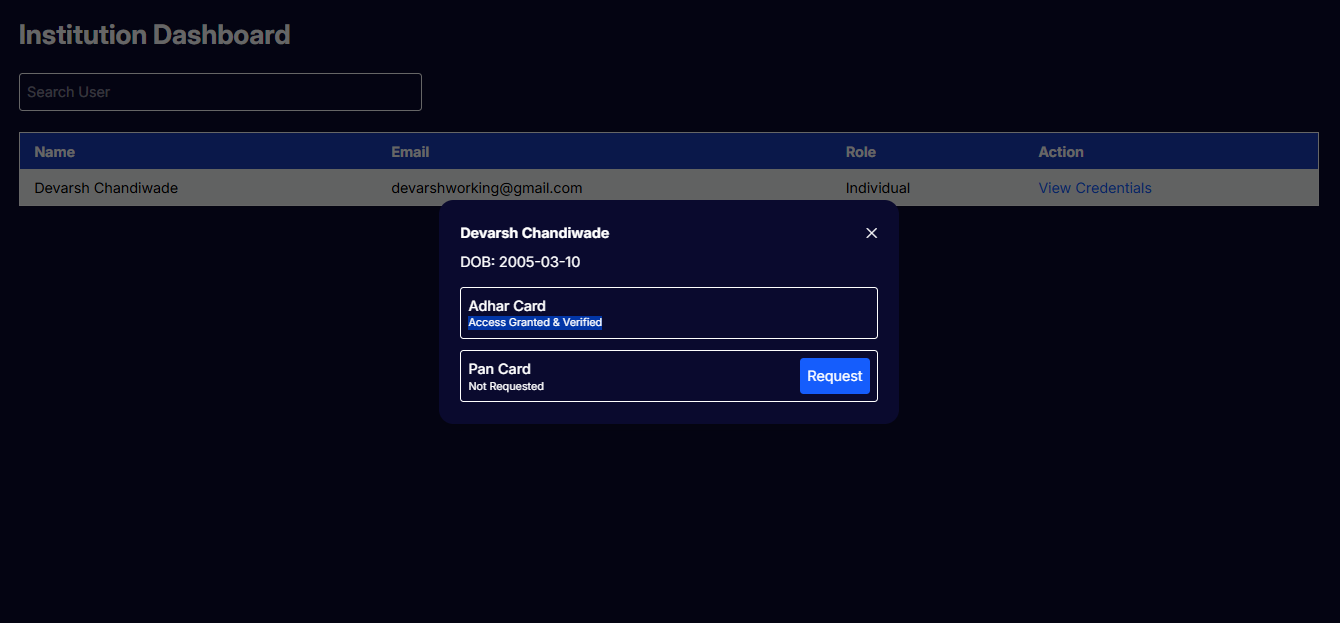
\includegraphics[width=0.8\textwidth]{Chapter1/ss5.png} % Adjust the width as needed
    \caption{Institution Verification Confirmation View}
    \label{f1} % Optional: for referencing the figure in your document
\end{figure}

\begin{figure}[h!]
    \centering
    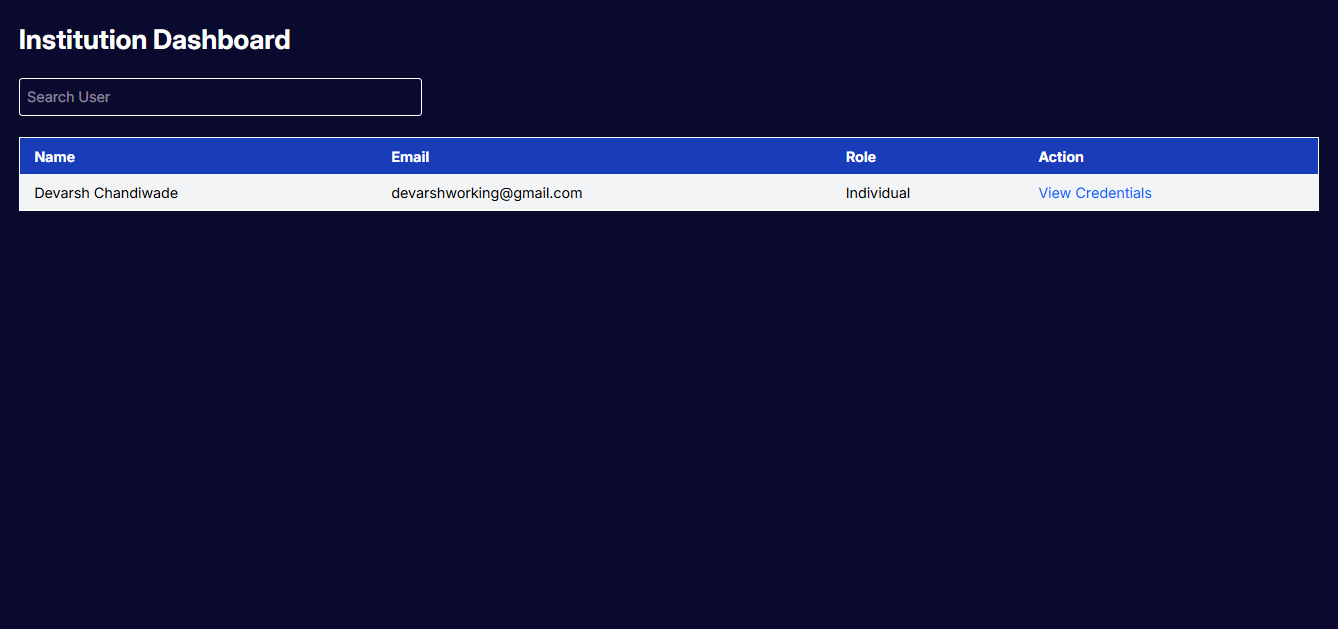
\includegraphics[width=0.8\textwidth]{Chapter1/ss6.png} % Adjust the width as needed
    \caption{Institution View of Verified Identity Status}
    \label{f1} % Optional: for referencing the figure in your document
\end{figure}


\chapter{Conclusions \& Future Scope}

\clearpage 
\chapter[Conclusions \& Future Scope]{Conclusions \& Future Scope}{Conclusions \& Future Scope}\label{res}

\noindent
\rule{0.49\textwidth}{0.75pt} $_{\bigcirc}$ \rule{0.49\textwidth}{0.75pt}\\
\section{Conclusions}
TrustChain offers a viable solution to safe identity verification by avoiding the process of exchanging uncoded personal data. The system allows users to be in total control of their identity and the institutions to do verification using proof based mechanisms. This minimizes the risks involved in exposing and abusing data.

Decentralized technologies like blockchain and IPFS provide the necessary transparency, immutability and reliability in identity management. Zero Knowledge Proofs help to enhance privacy by authenticating values without providing sensitive information. This is in line with the current security and data protection needs.

The system also initiates user controlled access management where the permissions could be granted or denied any time. Guardian based recovery can further increase reliability and guardian based recovery can guarantee continuity in case of key loss. This renders the platform to be secure and user friendly.

TrustChain, in general, exhibits a scalable and effective identity verification solution in the real world. It effectively changes the paradigm of sharing data to proving based validation, suitable in its adoption in various fields that need identity management.

It lays a robust basis of trust in online communications without invading users privacy. The strategy is in line with the new global requirements of decentralized identity systems. It also shows how cryptographic techniques can be applied in resolving real world security issues. It makes TrustChain a visionary solution in the changing world of digital identity management.
\noindent
\begin{center}
\rule{0.45\textwidth}{0.75pt} \; $\bigcirc$ \; \rule{0.45\textwidth}{0.75pt}
\end{center}

%\chapter{Conclusions \& Future Scope}



\section{Future Scope}
TrustChain may be expanded by means of connecting with official government databases like UIDAI and ITD to enhance the validity of document authentications. This would facilitate the real time validation of credentials and will increase trust into the system in the institutional use cases. 

In addition, enhanced recovery features like managed wallets and encrypted backups may be included. These upgrades will make them easier to use and less reliant on manual recovery processes and also enhance security.

Other technologies that can be integrated into the system include computer vision to verify documents automatically and extract data. This would assist in authenticating the authenticity of uploaded credentials and lessen reliance on third-party verification measures.

Moreover, large scale deployment can be investigated with scalability and performance optimizations. Increasing interoperability with the current digital identity platforms, as well as raising the user experience, will also contribute to the adoption of TrustChain in practical use.



\clearpage 
\include{Chapter1/Chapter10}
\clearpage 




% new chapters 
%\include{Chapter3/chapter3} 
%\include{Chapter4/chapter4}

\end{spacing}


%%% Note that if you want to add more chapters, which might be needed for showing another/more contributory chapters, make a copy of any folder of Chapter2/3 and rename it and include before including the conclusion.

% \renewcommand{\chaptername}{Chapter} %%%%%%%%%%%%%%%%%%%%%%%%%%%%
%
%    \addcontentsline{toc}{chapter}{Index} % added by Sandipan for registering 'Index' in the table of contents
%    \clearpage{\pagestyle{empty}\cleardoublepage}
%    \printindex       % added by Sandipan for printing the index
%    \renewcommand{\chaptername}{Chapter}

% \cmt{
% \renewcommand{\chaptername}{Appendix} %%%%%%%%%%%%%%%%%%%%%%%%%%%%
% \begin{spacing}{1}
% \begin{appendix}
% %%%%%%%%%%%%%%%%%%%%%%%%%%%% APPENDIX %%%%%%%%%%%%%%%%%%%%%%%%%%%%
% \include{Appendix/Appen1} 
% %\include{Appendix/Appen2} 
% %\include{Appendix/Appen3}
% % Atention!!! Include other appendixes if using this by copying  Appen1.tex file in the 'Appendix' folder before changing it.
% \clearpage{\pagestyle{empty}\cleardoublepage} 
% %%%%%%%%%%%%%%%%%%%%%%%%%%%%%%%%%%%%%%%%%%%%%%%%%%%%%%%%%%%%%
% \end{appendix}
% \end{spacing}
% }

\begin{appendix}
\include{Appendix/Appen1}
\end{appendix}

\clearpage{\pagestyle{empty}\cleardoublepage}
\renewcommand{\chaptername}{Chapter}
\addcontentsline{toc}{chapter}{References}
\chapter*{References}\label{ref}
\chaptermark{References}

\begin{thebibliography}{99}

\bibitem{1} Zaghdoudi, B., Bu, G., Potop-Butucaru, M., Fdida, S.: Blockchain-based decentralized iden-tity system: design and security analysis. In: 21st International Conference on Distributed Computing in Smart Systems and the Internet of Things (DCOSS-IoT 2025), Lucca, Italy, pp. 261–265. IEEE (2025). https://doi.org/10.1109/DCOSS-IoT65416.2025.00044

\bibitem{2} Seidi, S., Abdellaoui, A.: Securing and ensuring the confidentiality of medical data in the era of decentralized technologies: a blockchain and self-sovereign identity-based approach. J. Netw. Syst. Manage. 33, 81 (2025). https://doi.org/10.1007/s10922-025-09960-x

\bibitem{3} Wu, F., Ye, A., Diao, Y., Zhang, Y., Chen, J., Huang, C.: TrustChain: a privacy protection smart contract model with trusted execution environment. Blockchain: Research and Appli-cations 6(4), 100296 (2025). ISSN 2096-7209. https://doi.org/10.1016/j.bcra.2025.100296

\bibitem{4} Diwan, P., Kashyap, T., Badhan, A.K., Painkra, M.S., Maurya, S., Agrawal, P.: TrustNet: decentralised identity verification and management system. In: 4th OPJU International Tech-nology Conference (OTCON 2025) on Smart Computing for Innovation and Advancement in Industry 5.0, Raigarh, India, pp. 1–5. IEEE (2025). https://doi.org/10.1109/OTCON65728.2025.11071164

\bibitem{5} Lifna, C., Khithani, N., Alve, K., Gambhire, V., Hande, A., Choubey, S.: Blockchain-based intelligent disbursement in national scholarship portal. IET Blockchain 4(4), 407–422 (2024). https://doi.org/10.1049/blc2.12092

\bibitem{6} Kılıç, A., Betin Onur, C., Onur, E.: PATS: let parties have a say in threshold group key sharing. IET Information Security, Article ID 7557514, 14 pages (2024). https://doi.org/10.1049/2024/7557514

\bibitem{7} Lakshmi, J.M., Prasad, K., Babu, P.S.A., Ch, R.: A decentralized approach for enhancing identity and access management through blockchain integration. In: IEEE 6th International Conference on Cybernetics, Cognition and Machine Learning Applications (ICCCMLA 2024), Hamburg, Germany, pp. 237–242. IEEE (2024). https://doi.org/10.1109/ICCCMLA63077.2024.10871512

\bibitem{8} Babrekar, D., Patel, D., Patkar, S., Lobo, V.B.: Blockchain-based digital locker using BigchainDB and interplanetary file system. In: 6th International Conference on Communica-tion and Electronics Systems (ICCES 2021), Coimbatore, India, pp. 950–956. IEEE (2021). https://doi.org/10.1109/ICCES51350.2021.9489028

\bibitem{9} Naik, N., Jenkins, P.: Governing principles of self-sovereign identity applied to blockchain-enabled privacy-preserving identity management systems. In: IEEE International Symposium on Systems Engineering (ISSE 2020), Vienna, Austria, pp. 1–6. IEEE (2020). https://doi.org/10.1109/ISSE49799.2020.9272212

\end{thebibliography}

\clearpage{\pagestyle{empty}\cleardoublepage}

%\clearpage{\pagestyle{empty}\cleardoublepage}
%\renewcommand{\chaptername}{Chapter}
%\clearpage{\pagestyle{empty}\cleardoublepage}
\renewcommand{\chaptername}{Chapter}
\addcontentsline{toc}{chapter}{References}
\chapter*{References}\label{ref}
\chaptermark{References}

\begin{thebibliography}{99}

\bibitem{1} Zaghdoudi, B., Bu, G., Potop-Butucaru, M., Fdida, S.: Blockchain-based decentralized iden-tity system: design and security analysis. In: 21st International Conference on Distributed Computing in Smart Systems and the Internet of Things (DCOSS-IoT 2025), Lucca, Italy, pp. 261–265. IEEE (2025). https://doi.org/10.1109/DCOSS-IoT65416.2025.00044

\bibitem{2} Seidi, S., Abdellaoui, A.: Securing and ensuring the confidentiality of medical data in the era of decentralized technologies: a blockchain and self-sovereign identity-based approach. J. Netw. Syst. Manage. 33, 81 (2025). https://doi.org/10.1007/s10922-025-09960-x

\bibitem{3} Wu, F., Ye, A., Diao, Y., Zhang, Y., Chen, J., Huang, C.: TrustChain: a privacy protection smart contract model with trusted execution environment. Blockchain: Research and Appli-cations 6(4), 100296 (2025). ISSN 2096-7209. https://doi.org/10.1016/j.bcra.2025.100296

\bibitem{4} Diwan, P., Kashyap, T., Badhan, A.K., Painkra, M.S., Maurya, S., Agrawal, P.: TrustNet: decentralised identity verification and management system. In: 4th OPJU International Tech-nology Conference (OTCON 2025) on Smart Computing for Innovation and Advancement in Industry 5.0, Raigarh, India, pp. 1–5. IEEE (2025). https://doi.org/10.1109/OTCON65728.2025.11071164

\bibitem{5} Lifna, C., Khithani, N., Alve, K., Gambhire, V., Hande, A., Choubey, S.: Blockchain-based intelligent disbursement in national scholarship portal. IET Blockchain 4(4), 407–422 (2024). https://doi.org/10.1049/blc2.12092

\bibitem{6} Kılıç, A., Betin Onur, C., Onur, E.: PATS: let parties have a say in threshold group key sharing. IET Information Security, Article ID 7557514, 14 pages (2024). https://doi.org/10.1049/2024/7557514

\bibitem{7} Lakshmi, J.M., Prasad, K., Babu, P.S.A., Ch, R.: A decentralized approach for enhancing identity and access management through blockchain integration. In: IEEE 6th International Conference on Cybernetics, Cognition and Machine Learning Applications (ICCCMLA 2024), Hamburg, Germany, pp. 237–242. IEEE (2024). https://doi.org/10.1109/ICCCMLA63077.2024.10871512

\bibitem{8} Babrekar, D., Patel, D., Patkar, S., Lobo, V.B.: Blockchain-based digital locker using BigchainDB and interplanetary file system. In: 6th International Conference on Communica-tion and Electronics Systems (ICCES 2021), Coimbatore, India, pp. 950–956. IEEE (2021). https://doi.org/10.1109/ICCES51350.2021.9489028

\bibitem{9} Naik, N., Jenkins, P.: Governing principles of self-sovereign identity applied to blockchain-enabled privacy-preserving identity management systems. In: IEEE International Symposium on Systems Engineering (ISSE 2020), Vienna, Austria, pp. 1–6. IEEE (2020). https://doi.org/10.1109/ISSE49799.2020.9272212

\end{thebibliography}

\clearpage{\pagestyle{empty}\cleardoublepage}

%\addcontentsline{toc}{chapter}{References}
%\chapter*{References}
%\chaptermark{References}
%%%%%%%%%\cmt{    
\clearpage{\pagestyle{empty}\cleardoublepage}
\addcontentsline{toc}{chapter}{List of Publications}
\chapter*{Publications}
\section*{Journals}

\begin{enumerate}
	
	\item 
11th International Conference on Information and Communication Technology for Intelligent Systems (ICTIS 2026) \textit{(held in Bangkok, Thailand)}
	

\end{enumerate}

% \section*{Conferences}


% \begin{enumerate}

% 	\item One
% 	\item Two 
% 	\item Three

% \end{enumerate}


\noindent
\rule{0.49\textwidth}{0.75pt} $_{\bigcirc}$ \rule{0.49\textwidth}{0.75pt}\\








\clearpage{\pagestyle{empty}\cleardoublepage}
%%%%%%%%%%%%%%%%%}
%\begin{spacing}{1.25}
%\addcontentsline{toc}{chapter}{Author's Biography}
%\include{HeadTail/biodata}
%\clearpage{\pagestyle{empty}\cleardoublepage}
%\end{spacing}

\end{document}

